\section{Resultate}
In diesem Kapitel werden die Resultate der durchgeführten Untersuchungen aufgeführt.

\subsection{Ergebnisse des Modelltrainings} \label{chap:ergebnisse-modelltraining}
Beim Modelltraining wurden keine Erfolge mit den VGG- und AlexNet-Modellen erzielt, da diese Modelle nach dem Training alles als positiv klassifizieren. Der ViT erzielte ebenfalls schlechte Ergebnisse beim COVID CXR-4 Datensatz, konnte jedoch den MRI Datensatz im Vergleich besser erlernen.

\begin{figure}[H]
    \centering
    \begin{subfigure}{0.49\linewidth}
        \centering
        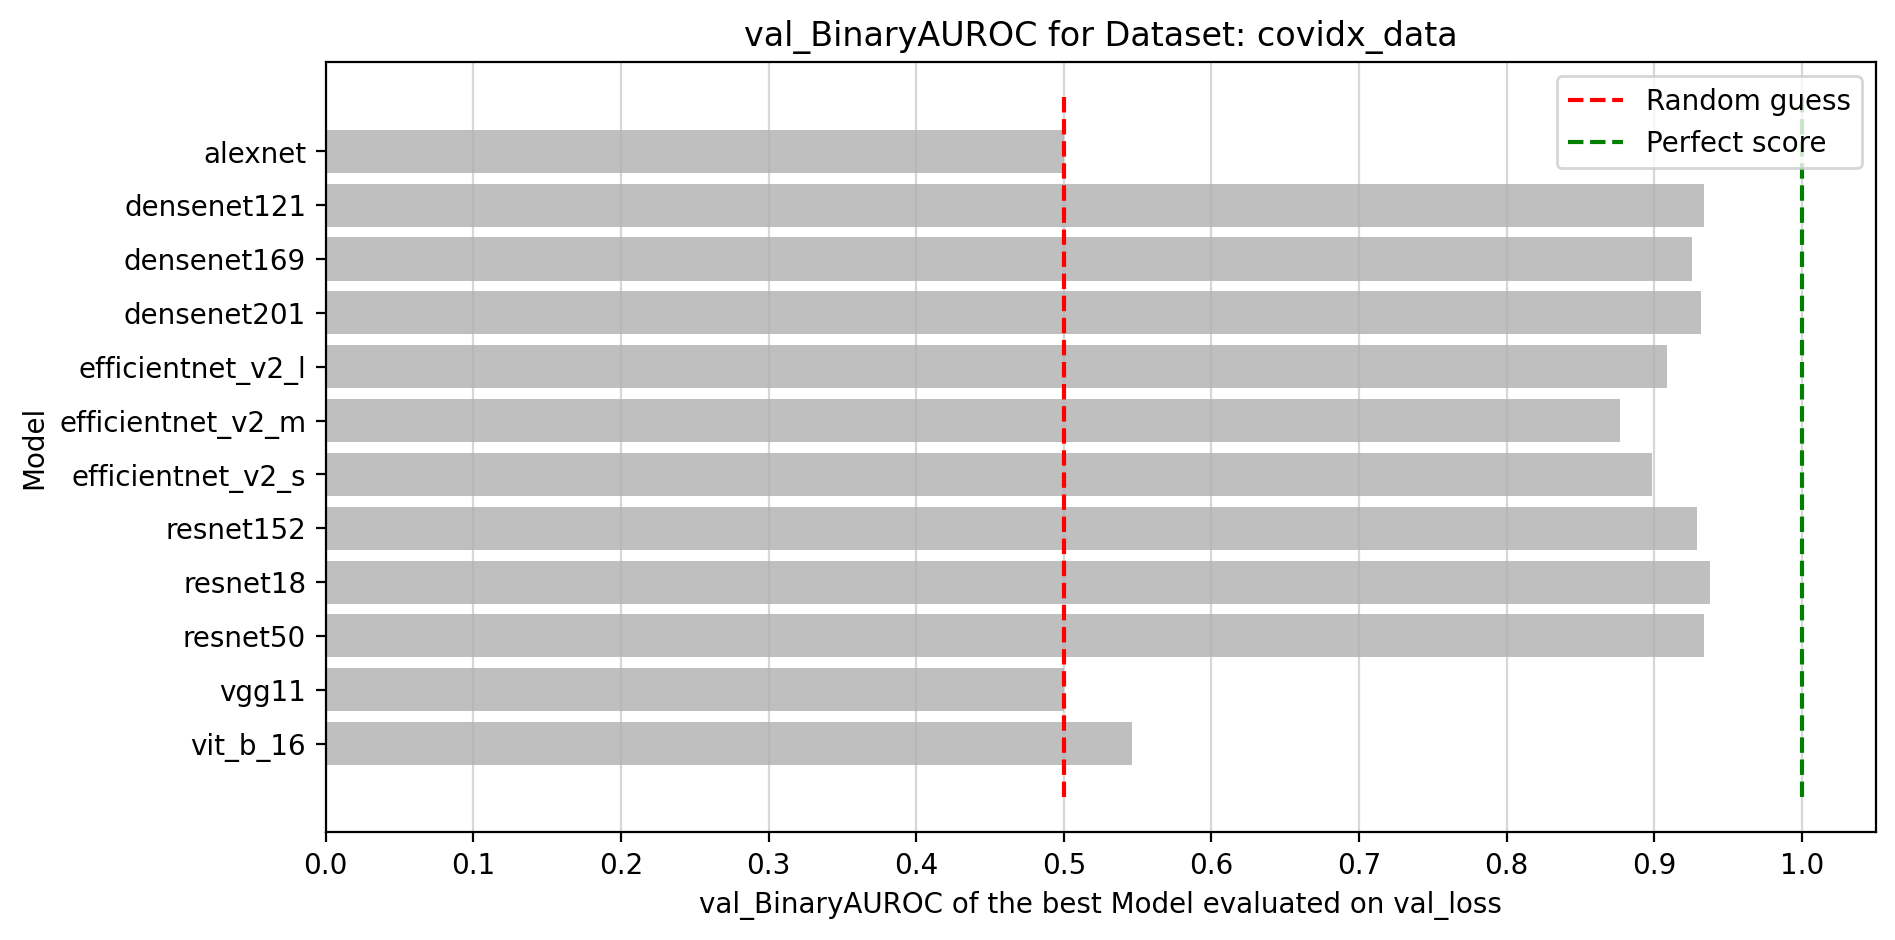
\includegraphics[height=0.49\linewidth]{01-images/05-resultate/val_binaryAUROC_COVIDX.png}
        \caption{AUROC Validierungsmetriken für den COVIDx CXR-4 Datensatz}
    \end{subfigure}\hfill%
    \centering
    \begin{subfigure}{0.49\linewidth}
        \centering
        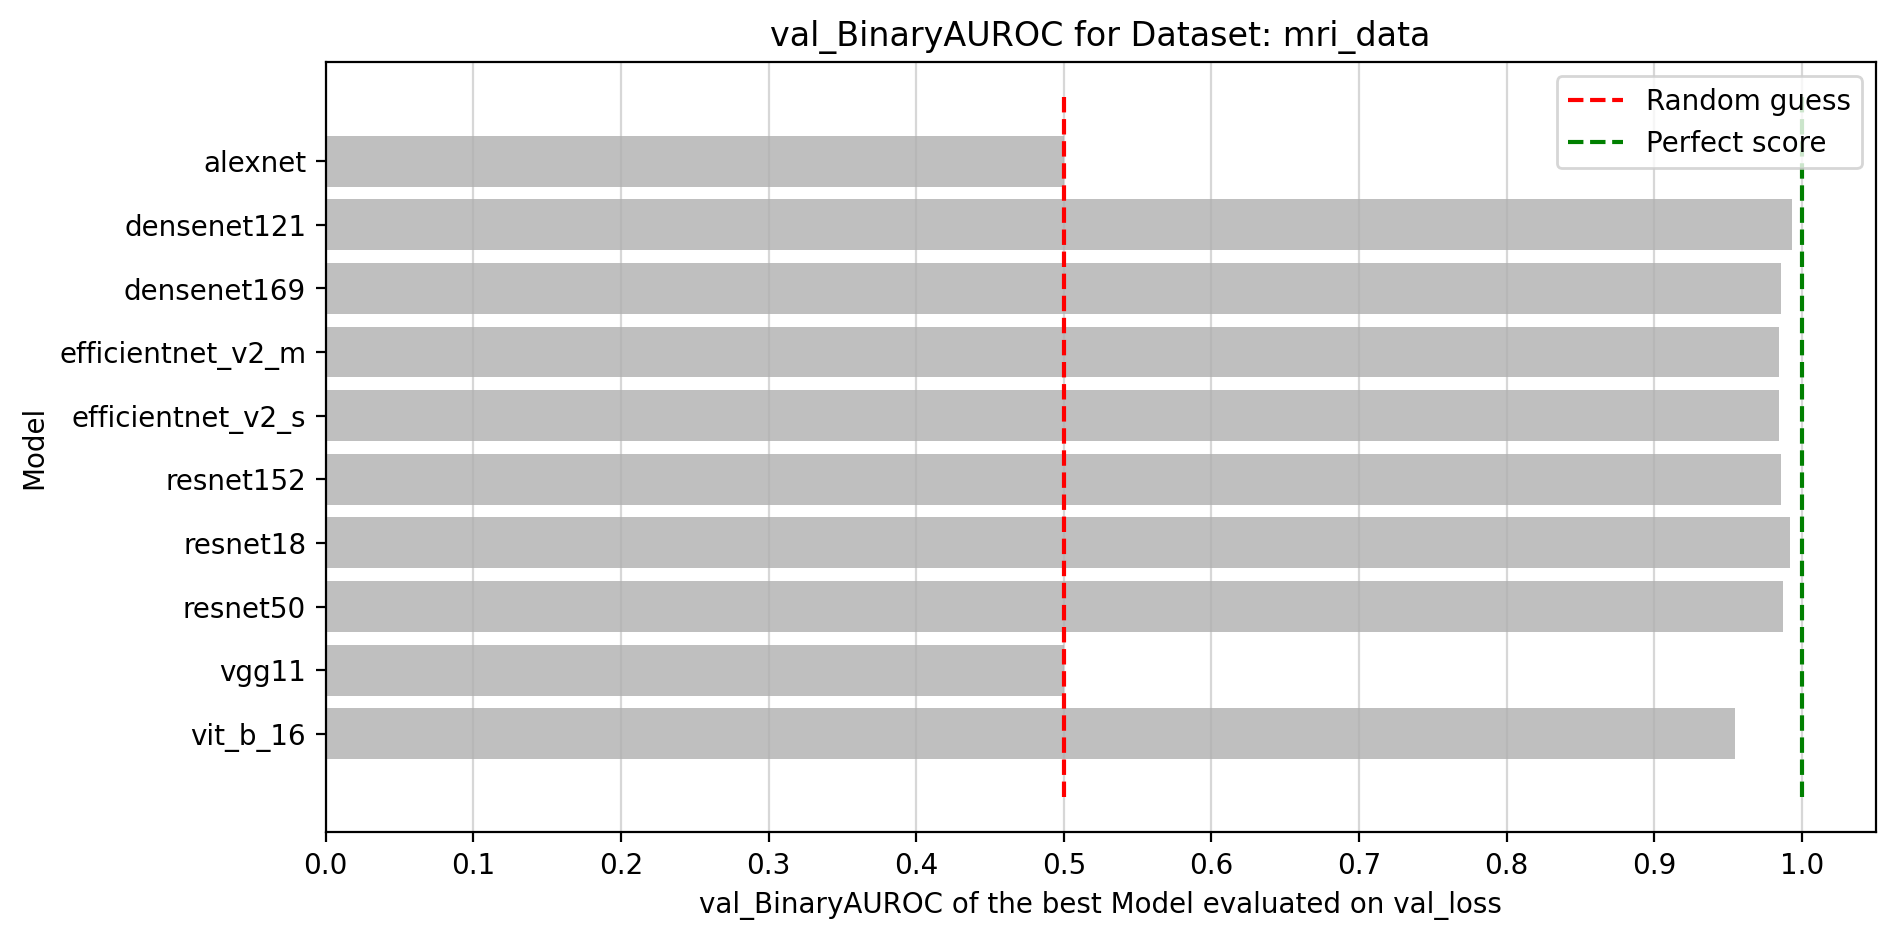
\includegraphics[height=0.49\linewidth]{01-images/05-resultate/val_binaryAUROC_MRI.png}
        \caption{AUROC Validierungsmetriken für den MRI Datensatz}
    \end{subfigure}
    \caption{Die AUROC-Validierungsmetriken der besten Modelle im Trainingslauf, gemessen an der val\_loss-Metrik}
    \label{fig:result-val-train}
\end{figure}

Zwischen den Abbildungen \ref{fig:result-val-train} und \ref{fig:result-test-train} sind  Differenzen in den AUROC Validierungs- und Testmetriken zu erkennen. Es lässt sich jedoch feststellen, dass die Modelle auf den Validierungsdaten zu overfitten scheinen, obwohl beim Training lediglich die Lernrate optimiert und das beste Modell anhand des Validierungsloss ausgewählt wurde. Beim Training der Modelle wurden keine weiteren Regularisierungen eingesetzt. Die Differenz der Metriken könnten durch mögliche Unterschiede in den Verteilungen der Datenpartitionen, wie in den Kapiteln \ref{chap:COVID19-datenverteilung} und \ref{chap:brain-datenverteilung} erklärt werden. 

\begin{figure}[H]
    \centering
    \begin{subfigure}{0.49\linewidth}
        \centering
        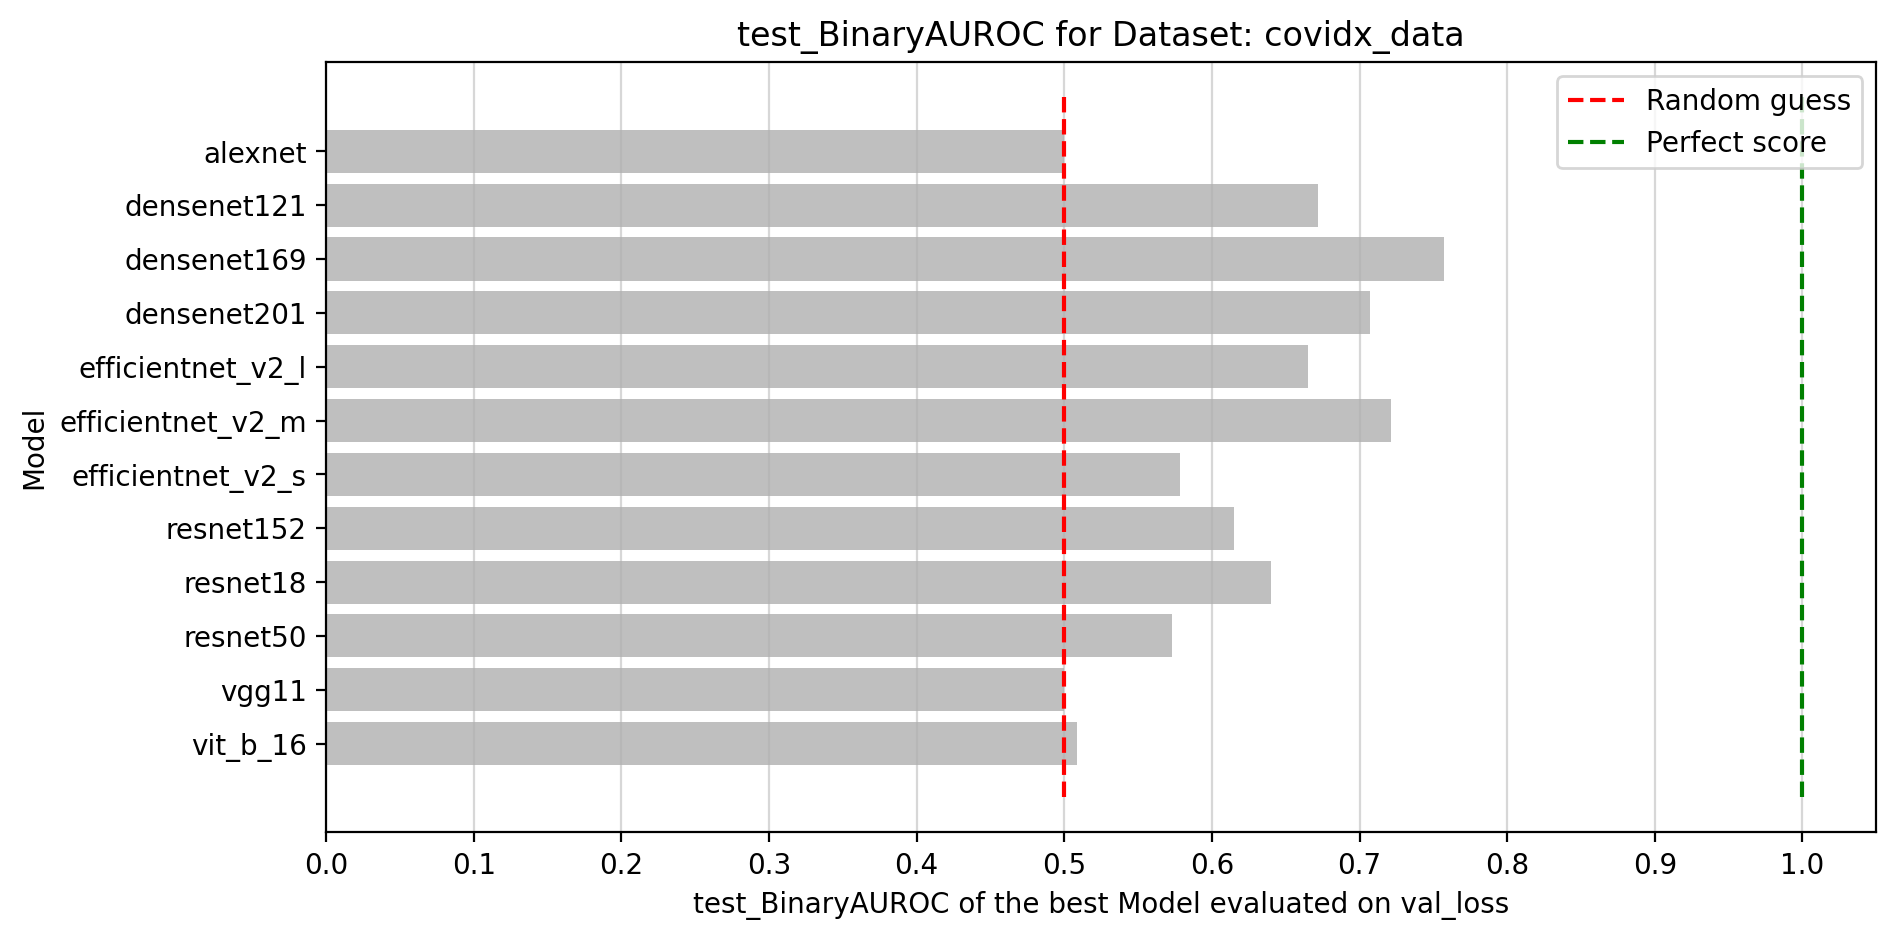
\includegraphics[height=0.49\linewidth]{01-images/05-resultate/test_binaryAUROC_COVIDX.png}
        \caption{AUROC Testmetriken für den COVIDx CXR-4 Datensatz}
    \end{subfigure}\hfill%
    \centering
    \begin{subfigure}{0.49\linewidth}
        \centering
        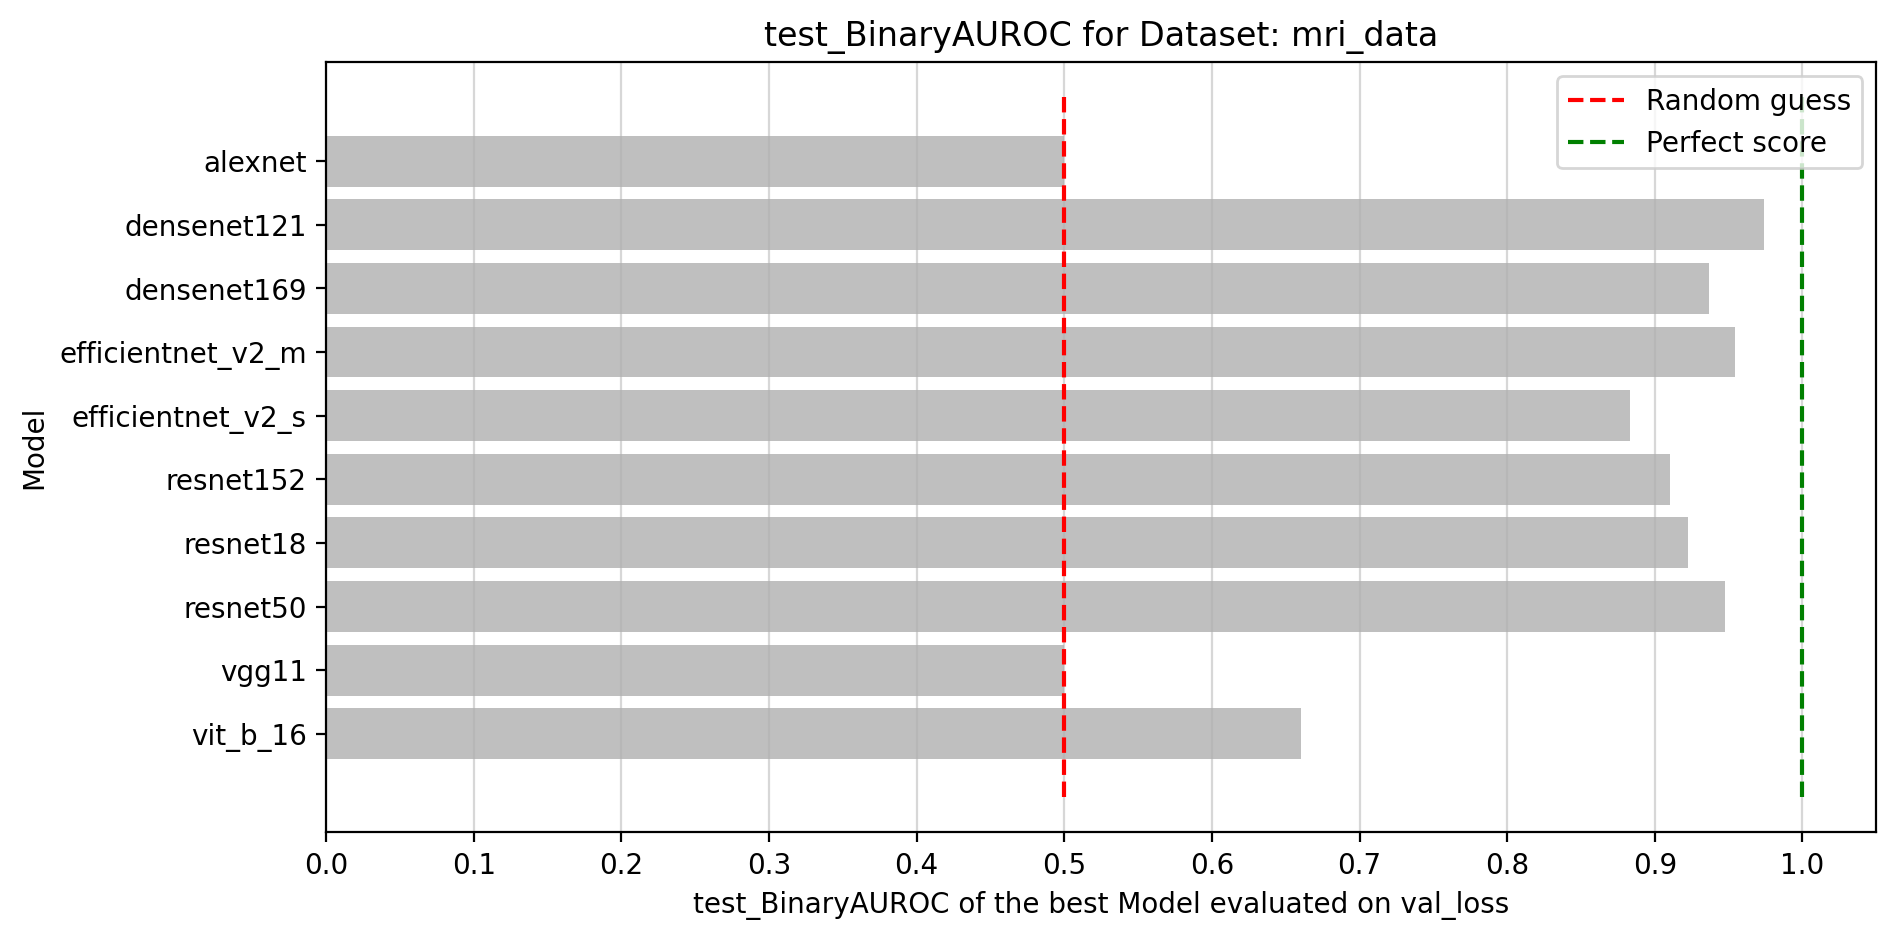
\includegraphics[height=0.49\linewidth]{01-images/05-resultate/test_binaryAUROC_MRI.png}
        \caption{AUROC Testmetriken für den MRI Datensatz\\\textcolor{white}{ich sehe dich}}
    \end{subfigure}
    \caption{Die AUROC-Testmetriken der besten Modelle im Trainingslauf, gemessen an der test\_loss-Metrik}
    \label{fig:result-test-train}
\end{figure}

Aufgrund der grossen Unterschiede zwischen dem Validierungs- und Testdatensatz erfolgt die Evaluation der Anfälligkeit der Modelle auf beiden Datensätzen. Die Metriken sind nicht optimal, jedoch ausreichend für die Bewertung des Robustifizierungsprozesses.

\newpage

